\documentclass[12pt,a4paper]{article}

\usepackage[left=3.00cm, right=2.00cm, top=2.00cm, bottom=2.00cm]{geometry}
\usepackage{lmodern}
\usepackage[T1]{fontenc}
\usepackage[utf8]{inputenc}
\usepackage[brazil]{babel}
\usepackage{microtype}

\usepackage{indentfirst,setspace}
\setlength{\parindent}{1.3cm}
\setlength{\parskip}{0.2cm}
\usepackage{enumitem}
\singlespacing

\usepackage{amssymb,amsmath,amsfonts}

\usepackage[num,overcite]{abntex2cite}
\citebrackets[]

\usepackage{longtable}
\usepackage{booktabs}
\usepackage[skip=1pt,labelfont=bf]{caption}
\usepackage{float}

\usepackage{array}

\usepackage{graphicx}
\graphicspath{ {./imgs/} }

\numberwithin{figure}{subsection}
\numberwithin{table}{subsection}

\usepackage{lipsum}

\author{Pablo Cecilio Oliveira\\
Marcilene Reis}
\title{Primeiro Trabalho Prático de AOC I\\
Assembly MIPS}
\date{}

\begin{document}
\maketitle

\section{Introdução}

Este documento apresenta a solução em MIPS para as duas questões do primeiro trabalho prático de Arquitetura e Organização de Computadores I.

\section{Implementação}

Toda a implementação foi realizada utilizando o programa de desenvolvimento MARS (\textit{MIPS Assembler and Runtime Simulator}) como IDE.

\subsection{Questão 1}

O procedimento para calcular o $cosseno$ de um ângulo segundo a série de Taylor abaixo:
\[ \cos x = \sum_{n=0}^{\infty} \frac{(-1)^n}{(2n)!} x^{2n} \]

A função $seno$ chama funções para calcular o fatorial e a função potência de $x$. O usuário digita o ângulo em radianos e a quantidade de termos da série ($n>0$).

\subsection{Questão 2}

O programa da Questão 2 recebe uma \textit{string} do arquivo de entrada (\texttt{entrada.txt}) e gera um arquivo de saída (\texttt{saida.txt}) contendo uma nova \textit{string} processada. O processamento da \textit{string} consiste na troca dos caracteres maiúsculos por minúsculos, e seus caracteres minúsculos por maiúsculos.

Para a implementação desse programa, uma lista de instruções e pseudo-instruções foi utilizada com o objetivo de simplificar o desenvolvimento.

\begin{itemize}[leftmargin=1.3cm]
\setlength\itemsep{1pt}
	 \item A pseudo-instrução {\ttfamily li} (\textit{Load Immediate}), carrega um valor imediato em um registrador.
	 \item A pseudo-instrução {\ttfamily la} (\textit{Load Address}), faz com que um registrador receba o valor de um ponteiro de outro local na memória.
	 \item A pseudo-instrução {\ttfamily move}, move o conteúdo de um registro para outro registro.
	 \item A instrução {\ttfamily lb} (\textit{Load Byte}), transfere um byte de dados de uma posição da memória principal para um registrador.
	 \item A instrução {\ttfamily sb} (\textit{Store Byte}), transfere um byte de dados de um registro para uma posição na memória principal.
\end{itemize}

As instruções do programa são listadas e comentadas abaixo:

Inicialmente, são declarados na área de segmento de dados do programa as variáveis a serem utilizadas e seus valores:

\begin{table}[H]
	\renewcommand{\arraystretch}{1}
	\centering
	\caption*{Área de declaração de variáveis}
	\label{q2cod:data}
	\begin{tabular}{>{\ttfamily}p{1.2cm} >{\ttfamily}p{4.6cm} p{9.2cm}}
	\toprule
	.data   & &  \\
	fin:    & .asciiz "entrada.txt" &  Endereço do caminho do arquivo de entrada.\\
	fout:   & .asciiz "saida.txt"   &  Endereço do caminho do arquivo de saída.\\
	string: & .space 1024 &  Reserva 1024 bytes para o \textit{buffer} que conterá a \textit{string}. \\
	\bottomrule
	\end{tabular}
\end{table}

Passa-se então a área de instruções {\ttfamily .text}, que contém os três procedimentos a serem realizados. A chamada para esses procedimentos é feita no escopo principal do programa ({\ttfamily main}):

\begin{table}[H]
	\renewcommand{\arraystretch}{1.2}
	\centering
	\caption*{Escopo principal do programa}
	\label{q2cod:main}
	\begin{tabular}{>{\ttfamily}p{4cm} p{11cm}}
		\toprule
		main:              & \\
		\midrule
		la \$a0,fin	       & Carrega o endereço de {\ttfamily fin} para a {\ttfamily \$a0}. \\
		jal leArquivo      & Inicia o procedimento {\ttfamily leArquivo}. \\
		la \$a0,string     & Carrega o endereço de {\ttfamily string} para a {\ttfamily \$a0}. \\
		jal manipulaString & Inicia o procedimento {\ttfamily manipulaString}. \\
		la \$a0,fout       & Carrega o endereço de {\ttfamily fout} para a {\ttfamily \$a0}. \\
		jal salvaArquivo   & Inicia o procedimento {\ttfamily salvaArquivo}. \\
		li \$v0,10         & \textit{load immediate} 10 em {\ttfamily \$v0} \\
		syscall            & Executa o número de serviço em {\ttfamily \$v0}. Terminar programa. \\
		\bottomrule
	\end{tabular}
\end{table}

Resumidamente o processo no {\ttfamily main} consiste em três partes:

\begin{enumerate}[leftmargin=1.3cm]
\setlength\itemsep{1pt}
	\item Abra o arquivo e carregue a \textit{string}; salve o numero de caracteres lidos.
	\item Manipule a \textit{string}; troque letras maiúsculas por minusculas e vice-versa.
	\item Salve para o arquivo; salva a \textit{string} modificada no arquivo de saída.
\end{enumerate}

Os procedimentos do programa são listados e comentados a seguir:

\begin{table}[H]
	\renewcommand{\arraystretch}{1.2}
	\centering
	\caption*{Procedimento para ler o arquivo}
	\label{q2cod:lefile}
	\begin{tabular}{>{\ttfamily}p{4cm} p{11cm}}
		\toprule
		leArquivo:       & \\
		\midrule[0.01cm]
		li \$v0,13       & Seta o número de serviço para a abertura de arquivo.  \\
		li \$a1,0        & Seta \textit{flag} = 0, \textit{read-only}. \\
		li \$a2,0        & modo ignorado \\
		syscall          & Executa o número de serviço em {\ttfamily \$v0}. Abrir arquivo. \\
		move \$t0,\$v0   & Salva o descritor do arquivo em {\ttfamily \$v0} para \ttfamily{\$t0}. \\
		\midrule[0.01cm]
		li \$v0,14       & Seta o número de serviço para a leitura de arquivo. \\
		move \$a0,\$t0   & Carrega o descritor do arquivo em {\ttfamily \$t0} para \ttfamily{\$a0}. \\
		la \$a1,string   & Carrega o endereço de {\ttfamily string} para a {\ttfamily \$a1}. \\
		li \$a2,255      & \textit{hardcoded buffer length} \\
		syscall          & Executa o número de serviço em {\ttfamily \$v0}. Ler arquivo. \\
		move \$s0,\$v0   & Salva o número de caracteres lidos em \ttfamily{\$s0} \\
		\midrule[0.01cm]
		li \$v0,16       & Seta o número de serviço para a fechar o arquivo. \\
		syscall          & Executa o número de serviço em {\ttfamily \$v0}. Fechar arquivo. \\
		\midrule[0.01cm]
		jr \$ra          & Retorna do procedimento \\
		\bottomrule
	\end{tabular}
\end{table}

\begin{table}[H]
	\renewcommand{\arraystretch}{1.2}
	\centering
	\caption{Tabela ASCII para A-Z e a-z}
	\label{tab:ascii}
	\begin{tabular}{rl|rl|rl|rl|rl|rl|rl}
		\toprule
		 65 & A &  69 & E &  73 & I &  77 & M &  81 & Q &  85 & U &  89 & Y \\
		 66 & B &  70 & F &  74 & J &  78 & N &  82 & R &  86 & V &  90 & Z \\
		 67 & C &  71 & G &  75 & K &  79 & O &  83 & S &  87 & W &     &   \\
		 68 & D &  72 & H &  76 & L &  80 & P &  84 & T &  88 & X &     &   \\
		\midrule
		 97 & a & 101 & e & 105 & i & 109 & m & 113 & q & 117 & u & 121 & y \\
		 98 & b & 102 & f & 106 & j & 110 & n & 114 & r & 118 & v & 122 & z \\
		 99 & c & 103 & g & 107 & k & 111 & o & 115 & s & 119 & w &     &   \\
		100 & d & 104 & h & 108 & l & 112 & p & 116 & t & 120 & x &     &   \\
		\bottomrule
		\multicolumn{12}{l}{\footnotesize Fonte: \citeauthor{wiki:xxx}}
	\end{tabular}
\end{table}

\begin{table}[H]
	\renewcommand{\arraystretch}{1}
	\centering
	\caption*{Procedimento para alterar a string}
	\label{q2cod:manipula}
	\begin{tabular}{>{\ttfamily}p{5cm} p{10cm}}
		\toprule
		manipulaString:        & \\
		\midrule[0.01cm]
		Loop:                  & loop para cada caractere da string \\
		lb \$t2,(\$a0)         & Aponta \$t2 para a posição de endereço de \ttfamily{\$a0} \\
		beq \$t2,\$zero,End    & Se \$t2 conter NULL, a string terminou, \ttfamily{End} \\
		slti \$t1,\$t2,90      & \$t2 e menor que 90(Z)? \\
		bne \$t1,\$zero,Upper  & Se \$t1 for 1 então 1 != 0, vai pra \ttfamily{Upper} \\
		slti \$t1,\$t2,122     & \$t2 e menor que 122(z)? \\
		bne \$t1,\$zero,Lower  & Se \$t1 for 1 então 1 != 0, vai pra \ttfamily{Lower} \\
		j Next                 & Va pra Next \\
		\midrule[0.01cm]
		Upper:                 & rotina para uppercase \\
		slti \$t1,\$t2,65      & \$t2 e menor que 65(A)? \\
		bne \$t1,\$zero,Next   & Se \$t1 for 1 então não é uma letra, \ttfamily{Next} \\
		addi \$t2,\$t2,32      & Soma 32 a \$t2 \\
		sb \$t2,(\$a0)         & armazena o valor na posição em \ttfamily{\$a0} \\
		j Next                 & Va pra Next \\
		\midrule[0.01cm]
		Lower:                 & rotina para lowercase \\
		slti \$t1,\$t2,97      & \$t2 e menor que 97(a)? \\
		bne \$t1,\$zero,Next   & Se \$t1 for 1 então não é uma letra, Next \\
		addi \$t2,\$t2,-32     & Soma -32 a \ttfamily{\$t2} \\
		sb \$t2,(\$a0)         & armazena o valor na posição em \ttfamily{\$a0} \\
		\midrule[0.01cm]
		Next:                  & Continua a interação \\
		addi \$a0,\$a0,1       & Incrementa o endereço de \ttfamily{\$a0} \\
		j Loop                 & Va para Loop \\
		\midrule[0.01cm]
		End:                   & Termino do Loop \\
		jr \$ra                & Retorna do procedimento \\
		\bottomrule
	\end{tabular}
\end{table}

\begin{table}[H]
	\renewcommand{\arraystretch}{1}
	\centering
	\caption*{Procedimento para salvar o arquivo}
	\label{q2cod:salvafile}
	\begin{tabular}{>{\ttfamily}p{4cm} p{11cm}}
		\toprule
		salvaArquivo:    & \\
		li \$v0, 13      & \textit{system call}: Abre o arquivo \\
		li \$a1, 1       & \textit{flag} para escrita \\
		li \$a2, 0       & modo ignorado \\
		syscall          & Abra o arquivo! \\
		move \$t0,\$v0   & Salva o \textit{descriptor} em \$t0 \\
		\midrule[0.01cm]
		li \$v0,15       & \textit{system call}: Escrevendo no arquivo \\
		move \$a0,\$t0   & Carrega o descriptor do arquivo \\
		la \$a1,string   & endereço do \textit{buffer} \\
		move \$a2,\$s0   & carrega \textit{strlen} de \$s0 \\
		syscall          & Escreva no arquivo! \\
		\midrule[0.01cm]
		li \$v0,16       & \textit{system call}: Fecha o arquivo \\
		syscall          & Feche o arquivo! \\
		jr \$ra          & Retorna do procedimento \\
		\bottomrule
	\end{tabular}
\end{table}

\pagebreak

\section{Estatísticas das instruções}

Os resultados fornecidos pela ferramenta de estatísticas de instruções do MARS são sumarizados para cada questão nas figuras abaixo:  

\begin{figure}[H]
	\centering
	\caption*{Questão 2, resultado da análise}
	\vspace{0.2cm}
	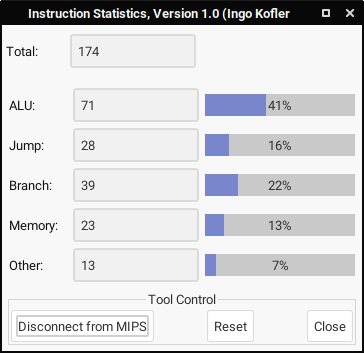
\includegraphics[width=242px]{questao2_stats}
	\\\footnotesize Fonte: Mars Instruction Statistic Tool
\end{figure}

\begin{flushleft}
	\bibliography{TP1}
	\vfill
	O histórico do desenvolvimento desse trabalho se encontra online em:\\ \url{https://github.com/Durfan/ufsj-aoc1-tp1}.
\end{flushleft}

\end{document}
